%\documentclass[reprint,aps,graphicx,pre,showpacs]{revtex4-1}
\documentclass{article}
\usepackage[margin=1.0in]{geometry}                % See geometry.pdf to learn the layout options. There are lots.
\usepackage{geometry}
%\geometry{landscape}                % Activate for for rotated page geometry
%\usepackage[parfill]{parskip}    % Activate to begin paragraphs with an empty line rather than an indent
\usepackage{euscript,amsmath,amssymb,amsfonts,graphicx,bm}
\usepackage{hyperref}
\hypersetup{colorlinks=true,linkcolor=blue,citecolor=red}
\usepackage{epstopdf}
\usepackage{enumerate}
\usepackage{csquotes}
\usepackage{caption}
\usepackage{subcaption}
\usepackage{mathrsfs}
\usepackage{xcolor}
\usepackage{lineno}
%\usepackage[nomarkers,figuresonly]{endfloat}
%\linenumbers


\newcommand{\bM}{{\bf M}}
\newcommand{\by}{{\bf y}}
\newcommand{\f}{{\bf f}}
\newcommand{\bg}{{\bf g}}
\newcommand{\bz}{{\bf z}}
\newcommand{\bZ}{{\bf Z}}
\newcommand{\bmu}{{\boldsymbol \mu}}
\newcommand{\bnu}{{\boldsymbol \nu}}
\newcommand{\bphi}{{\boldsymbol \phi}}


\usepackage{mathtools} % for \vcentcolon
%\usetikzlibrary{calc}
%\linespread{2}
\usepackage{amsthm}
%\numberwithin{equation}{section}
\usepackage{authblk}

\makeatletter
\renewcommand{\maketitle}{\bgroup\setlength{\parindent}{0pt}
\begin{flushleft}
  \textbf{\LARGE \@title}

  \@author
\end{flushleft}\egroup
}
\makeatother
%
\author[1]{Yeast DNA repair group}
%\author[2]{Jane Kondev}
%\author[3]{Ariel Amir}
%\affil[1]{Harvard, Pasteur, Peking }
%\affil[1,2]{Department of Physics, Brandeis University, Waltham, MA 02453 USA}
%\affil[3]{School of Engineering and Applied Sciences, Harvard University, Cambridge, MA 02138, USA}

\makeatletter
\patchcmd{\@maketitle}{\LARGE \@title}{\fontsize{20}{19.2}\selectfont\@title}{}{}
\makeatother

\renewcommand\Authfont{\fontsize{10}{14.4}\selectfont}
\renewcommand\Affilfont{\fontsize{9}{10.8}\itshape}

\newtheorem{thm}{Theorem}[section]
\newtheorem{defn}{Definition}[section]
\newtheorem{lem}{Lemma}[section]
\newtheorem{cor}{Corollary}[section]
\newtheorem{prop}{Proposition}[section]
 \newtheorem{ass}{Assumption}



%\newcommand[1]{\ensuremath{#1}}
% \makeatletter
%\renewcommand{\email}[2][]{%
%  \ifx\emails\@empty\relax\else{\g@addto@macro\emails{,\space}}\fi%
%  \@ifnotempty{#1}{\g@addto@macro\emails{\textrm{(#1)}\space}}%
%  \g@addto@macro\emails{#2}%
%}
%\makeatother
%
% \usepackage{amsaddr}



\title{Dynamics of double-strand break and repair in growing populations}
\date{\today}
\begin{document}


\maketitle
\tableofcontents

\section{Introduction}

\section{Analysis of pooled data reveals time-scales of break and repair}
We begin by ignoring the single-cell resolution afforded to us by the individual wells, and treat each condition as a bulk experiment by studying the number of bright field and GFP cells averaged over all the wells. The trajectories of the average number of bright field and GFP cells are shown in Figure \ref{fig:1} (A). We compare this data to a simple ODE mode in which an initial population of cells with modified DNA grows at a rate $\alpha$ and switches into a non-growing, broken state, at a rate $\rho$. The broken cells can then become repaired and once again begin to grow at a rate $\alpha$. Letting $m$, $b$ and $g$ be the number of modified, broken and repaired (or green) cells, we have
\begin{align}\label{mbg_ode}
\frac{d}{dt}m &= (\alpha - \beta) m\\
\frac{d}{dt}b &= \beta m - \rho b\\
\frac{d}{dt}g &= \alpha g + \rho b.
\end{align}
It is easy to see that the total population size $n = m+b+g$ will eventually grow exponentially at a rate $\alpha$. We can therefore obtain $\alpha$ by fitting the bright field data to an exponential. We can also see from these equations that $m$ and $b$ will eventually grow (assuming $\alpha> \beta$) exponentially at a rate $\alpha-\beta$, while $g$ will eventually grows at a rate $\alpha$. 
Therefore, a prediction of this model is that the fraction of  non-GFP cells, $\phi_{m+b} = (b+m)/(m+b+g)$  decays exponentially at a rate $\beta$:
\begin{equation}
\phi_{m+b} \sim 1- e^{-\beta t}. 
\end{equation}
Note that this result is independent of whether we impose a carrying capacity on the population, the ratios will remain unchanged even if the population is not growing exponentially. 
Fitting $\ln (1-\phi_{m+b})$ to a line thus gives us a way to infer the break rate which (at least in the long-term) is independent of $\rho$. 
This exponential decay is seen in some, but not all experiments; see Figure \ref{fig:1} (B). In CTG-Cpf1 and CGG-Cpf1 the green cells appear very slowly, making is difficult to separate the long term decay from the the transient dynamics. In GAA-SpCas9 and CTG-SpCas9 we don't see the number of GFP cells converge to the number of bright field cells, resulting an a biphasic trajectory of $\phi_{m+b}$. 

\begin{figure}[h!]
\centering
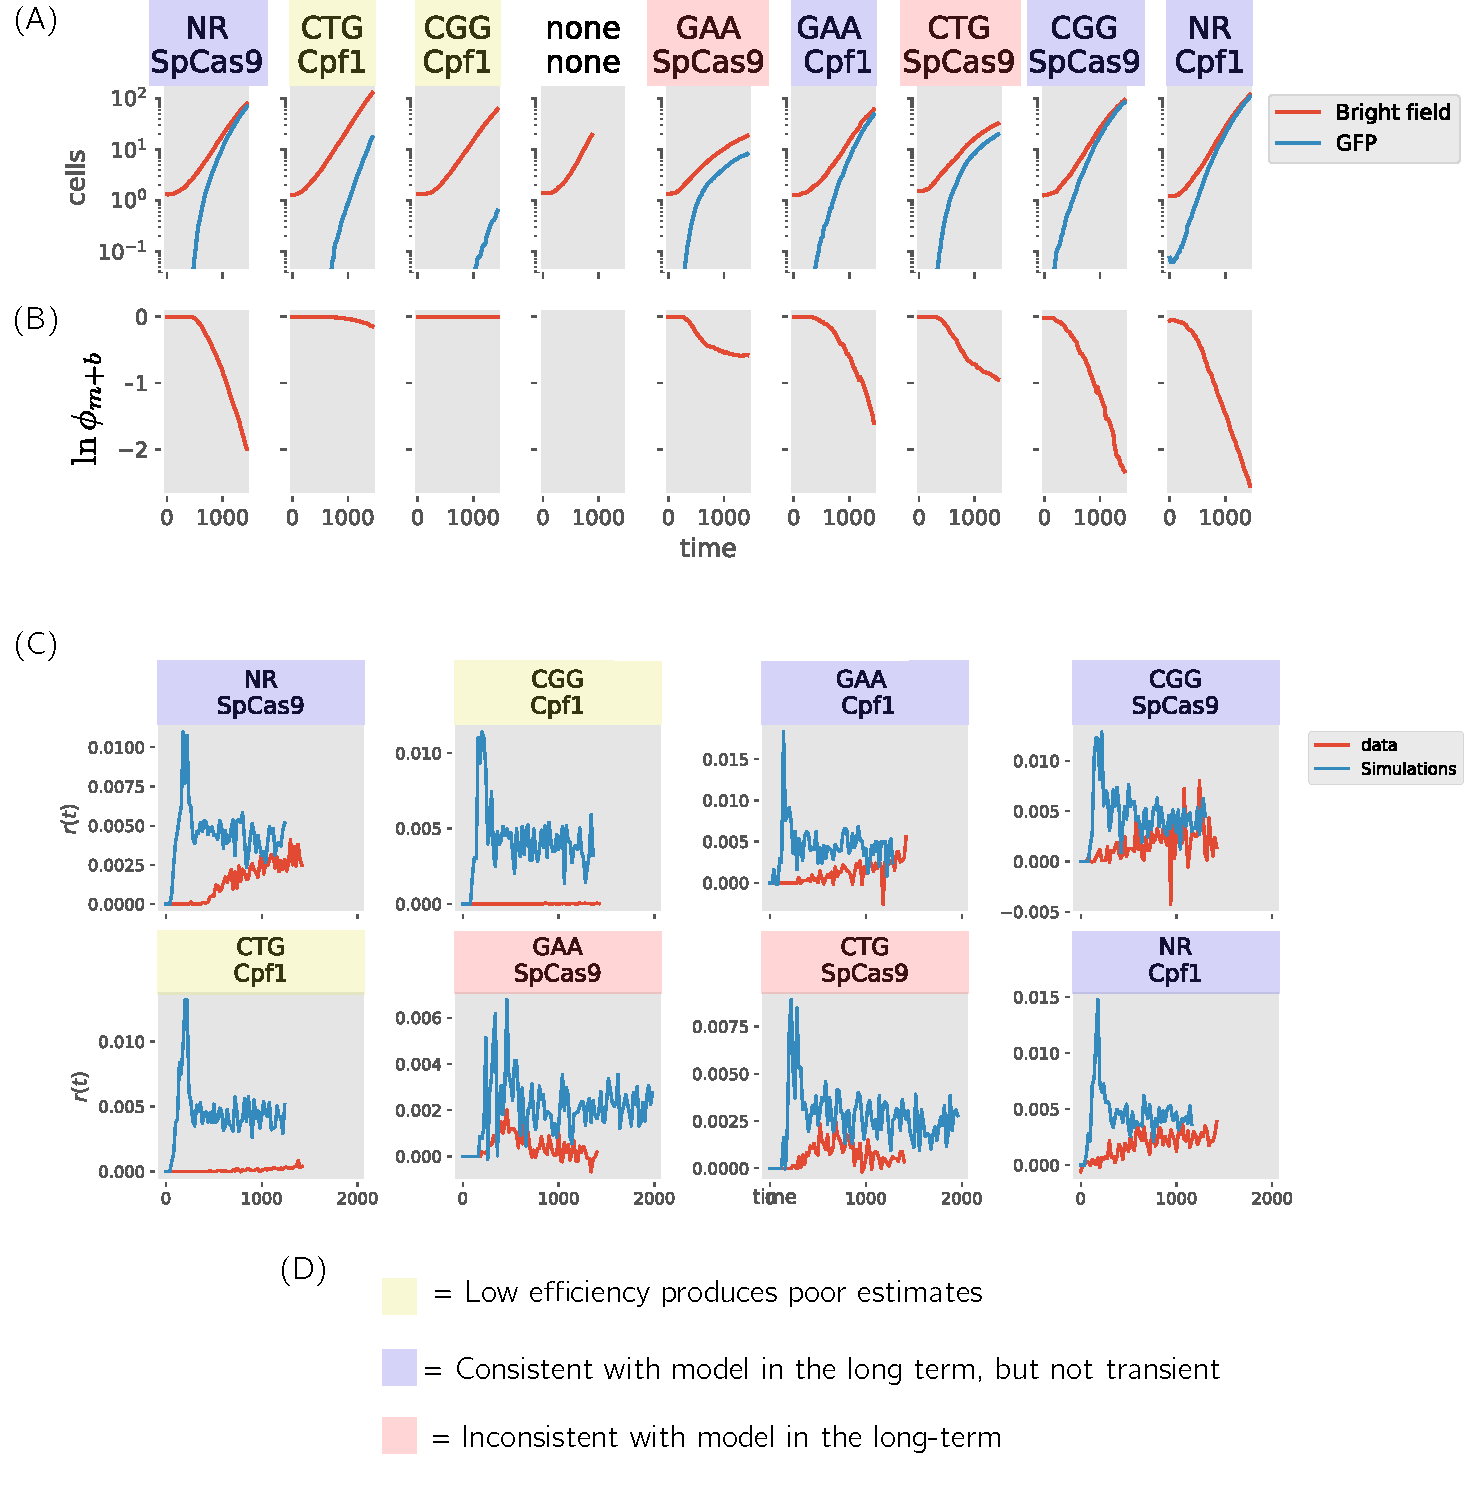
\includegraphics[scale=0.6]{fig1.pdf}
\caption{(A) The average number of bright field and GFP cells as a function of time in each condition.  (B) The fraction of non-GFP cells as function of time for each condition.  (C) The rate to turn green obtained from Equation \ref{rt} compared to simulations of the model without a broken state using values of inferred from the trajectories in (B). Classification of experiments in terms of comparison between predictions from (B) and (C). }\label{fig:1}
\end{figure}


An alternative approach to inferring $\beta$ is to look at the instantaneous  production of green cells. Solving for $\beta$ in Equation \ref{mbg_ode}, we get 
\begin{align}
\begin{split}
\beta &= \frac{1}{m}\left[\frac{d}{dt}b +\rho b\right] =  \frac{1}{m}\left[\frac{d}{dt}b +\frac{d}{dt}g - \alpha g\right] \\
&= \frac{1}{n-g-b}\left[\frac{d}{dt}b +\frac{d}{dt}g -\frac{g}{n-b} \frac{d}{dt}n\right]
\end{split}
\end{align}
Since we don't know the number of broken and not yet repaired cells, we can't compute all the terms in this equation directly. Intuitively, if $\rho \gg \beta$, we can neglect the broken cells \textcolor{red}{[I believe this is usually called an adiabatic  approximation]}, leading to the approximation
\begin{equation}\label{rt}
\beta \approx r(t) \equiv \frac{1}{n-g}\left[\frac{d}{dt}g -\frac{g}{n} \frac{d}{dt}n\right]. 
\end{equation}
Within the model, we can obtain an exact formula for $r(t)$ for finite $\rho$ by plugging the solution of Equation \ref{mbg_ode} into Equation \ref{rt} (see Appendix \ref{app:ode}).  We find that if $\beta < \alpha$, $r(t) \to \beta$ in the long-time limit, regardless of $\rho$. 


In Figure \ref{fig:1} (C) we compare $r(t)$ compute for the data and simulations of the model with $\rho \to \infty$ so that there are no broken cells. We first focus on the experiments for which $\phi_{m+b}$ exhibits clear exponential decay. For these experiments, the simulations and data appear to be converging to similar values of $r(t)$, although the transient dynamics different significantly. Since the convergence of $r(t)$ to $\beta$ depends on $\rho$, we check whether the trajectories can be reproduced by simulations of the model with finite $\rho$. Selecting values of $\rho$ on the order of $\beta$, we find that the qualitative features of the trajectories are reproduced; see  Figure \ref{fig:2} (B). However, this does not explain the ``bump" in the CAA-SpCas9 and CTG-SpCas9. To reproduce this, we assume that some fraction of the repaired cells fail to turn green, but still grow. A simulation of this model is shown in Figure \ref{fig:2} (B), where we can see that this will indeed produce the behavior observed in some experiments. 


\begin{figure}[h!]
\centering
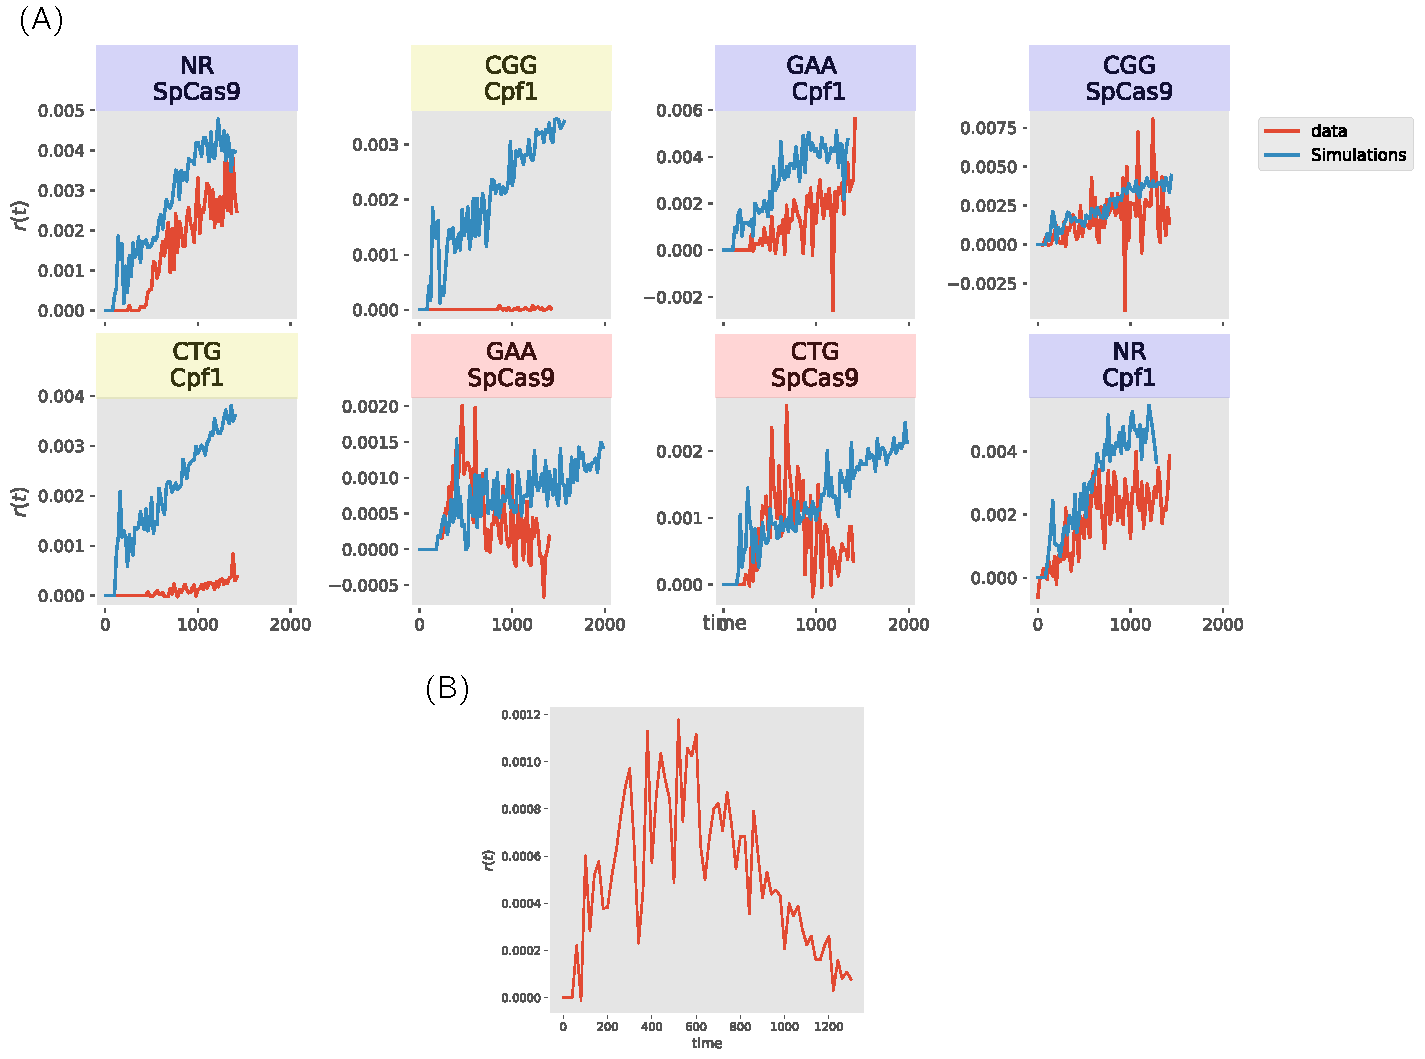
\includegraphics[scale=0.6]{fig2.pdf}
\caption{ (C) The rate to turn green obtained from Equation \ref{rt} compared to simulations of the model with a broken with the values of $\alpha$ and $\beta$ inferred from the trajectories in Figure \ref{fig:1} (B) and values of $\rho$ comparable to $\beta$. (B) A simulation of the model with $1/2$ of the repaired cells failing to turn green.  }\label{fig:2}
\end{figure}


\section{Inference from ODE model predicts well-to-well variability}

\begin{figure}[t!]
\centering
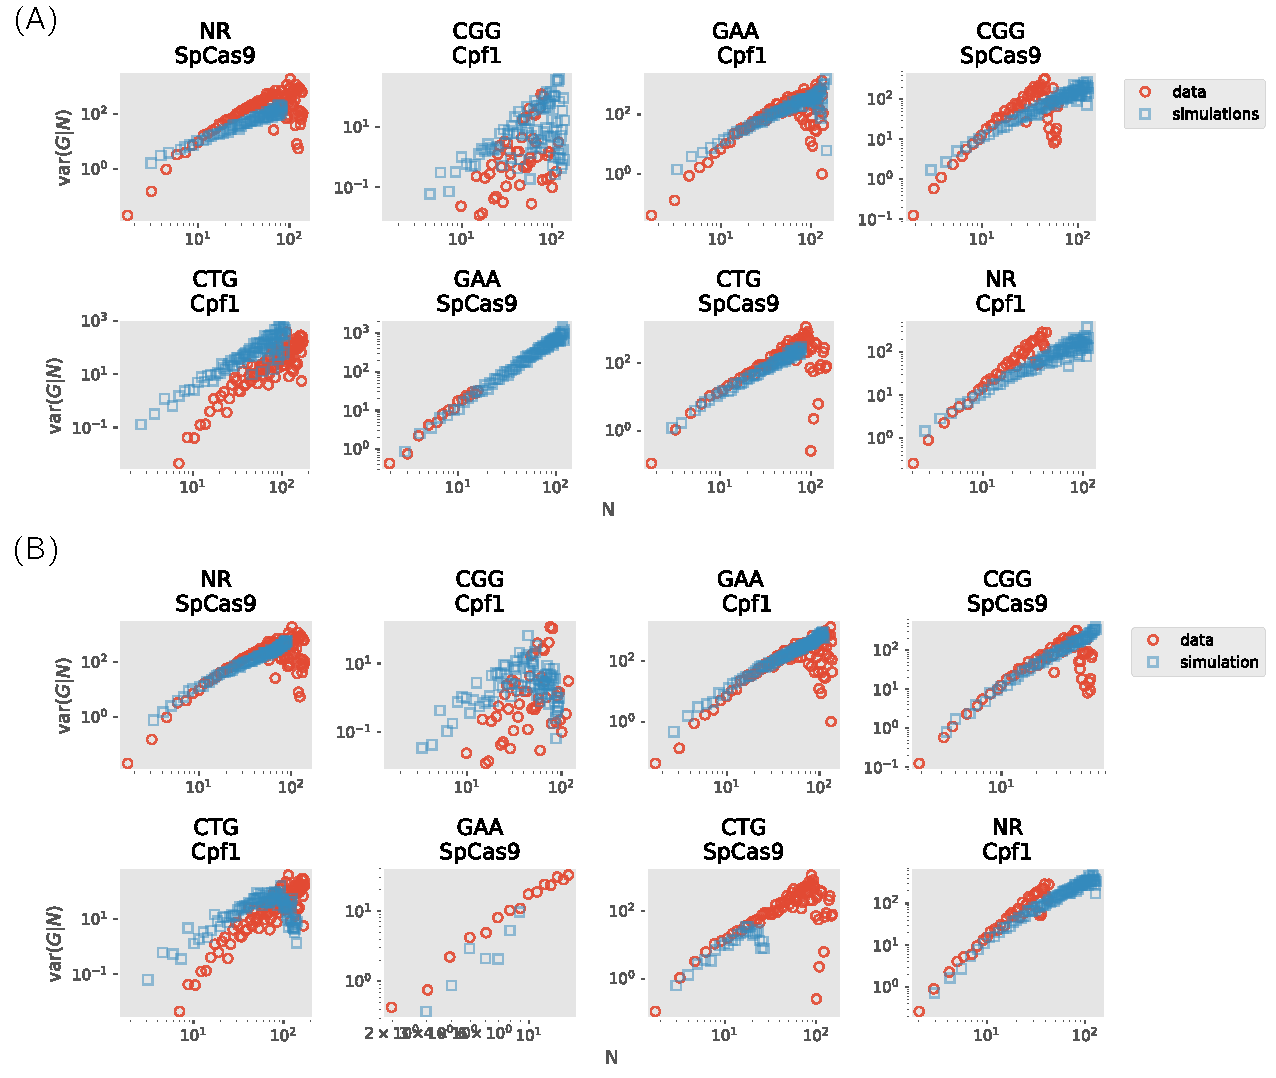
\includegraphics[scale=0.7]{fig3.pdf}
\caption{(A) ${\rm var}(G|N)$ compared to simulations of the constant probability model with parameters computed from the previous section.   (B) The same as (A) but including a broken state. }\label{fig:3}
\end{figure}

We now consider the variability between wells within a condition. In order to remove the effects of lag time and asynchronous  growth, we consider the variance  of $G$ conditioned on the total number of cells, ${\rm var}(G|N)$. In a simple model where we neglect the broken, non-green state, ${\rm var}(G|N)$ undergoes phase transition at $p_c = 1/2$ (see Section \ref{app:sync} for derivation). When $p<1/2$, ${\rm var}(G|N)$ grows exponentially, while for $p<1/2$ it decays. In all the experiments, we find that ${\rm var}(G|N)$ grows exponentially. The growth of ${\rm var}(G|N)$ is given by the formula 
\begin{equation}
{\rm var}(G_t|N) = \left\{\begin{array}{cc} 
\frac{p}{1-2p} N^{2 + 2 \ln(1-p)/\ln(2)}& \text{ if } p<1/2\\
\frac{p}{2p-1} N^{1+ 1 \ln(1-p)/\ln(2)}& \text{ if } p>1/2
\end{array}\right.
\end{equation}
This formula seems to be fairly accurate for a more realistic asynchronous model where cells have generation times drawn from a distribution.  Interestingly, the inclusion of a broken state does not affect the long-term behavior of ${\rm var}(G_t|N_t)$; see Section \ref{app:sync}. In Figure \ref{fig:3}, we compare the fluctuations in the data to those in simulations of the the random generation time model  \textcolor{red}{[Need to define this somewhere]} using parameter values computed from Figure \ref{fig:1} as described in the previous section. We simulate the model both with and without the broken state and see that the broken state model does a slightly better job of predicting the growth of the fluctuations, suggesting the broken state is indeed important. However, there are still some inconsistencies between the simulations and the data; namely, the decrease in ${\rm var}(G|N)$ at the end of the experiment.  


\textcolor{red}{To-do: 
\begin{itemize}
\item Test if lag between repair and GFP production (but no broken state) can also reproduce qualitative features of data
\item Find more quantitive way to infer $\rho$ (currently just tried $\rho$ close to $\beta$). Fitting the curves doesn't work so well due lag time. 
\item Plot variance in green cells as a function of time in data vs. simulations
\end{itemize}
}



\newpage

\appendix

\renewcommand{\theequation}{S.\arabic{equation}}

\section{Solution of ODE model}\label{app:ode}
The ODEs given in Equation \ref{mbg_ode} can be solved explicitly as follows. First note that the equation for $m$ is decoupled from the other three, and has the solution 
\begin{equation}
m(t) = m(0)e^{t(\alpha-\beta)}.
\end{equation}
The equation for $b(t)$ can then be solved using an integrating factor. With $b(0) = 0$, this leads to 
\begin{equation}
b(t) = \frac{\beta  m(0) \left(e^{t (\alpha -\beta)}-e^{-\rho t}\right)}{\alpha -\beta +\rho }.
\end{equation}
Doing the same for $g(t)$ yields
\begin{equation}
g(t) =\frac{m(0) \rho  \left(\beta e^{-\rho t} -(\alpha +\rho ) e^{t (\alpha -\beta)}+(\alpha -\beta +\rho ) e^{t \alpha }\right)}{(\alpha +\rho ) (\alpha -\beta +\rho )}.
\end{equation}
Plugging the solutions for $b(t)$, $m(t)$ and $g(t)$ into $r(t)$ yields (after some simplification)
\begin{equation}
r(t) =\frac{\beta  \rho ^2 e^{t (\beta +\rho )} \left(\alpha  \beta  e^{t (\alpha +\beta +\rho )}+\beta  \rho  e^{t (2 \alpha +\rho )}-\beta 
   (\alpha +\rho ) e^{t (\alpha +\beta )}+(\alpha -\beta ) (\alpha +\rho ) e^{t (\alpha +\rho )}-\alpha  e^{\alpha  t} (\alpha -\beta +\rho
   )+\beta  \rho  e^{\beta  t}\right)}{\left(\rho  e^{t (\alpha +\rho )}+\beta  e^{t (\beta +\rho )}+\beta  \left(-e^{\beta  t}\right)\right)
   \left(\alpha ^2 \beta  \left(-e^{\beta  t}\right)+\beta  \rho ^2 e^{t (\alpha +\beta +\rho )}-\beta  (\rho -\alpha ) (\alpha +\rho ) e^{t
   (\beta +\rho )}+\alpha  \rho  (\alpha +\rho ) e^{t (\alpha +\rho )}\right)}.
\end{equation}
We can obtain the large time limit by looking at the fastest growing terms in the numerator and denominator. If $\alpha> \beta$ (which is true for all experiments) the fastest growing terms grow exponentially with rates $2\alpha + \beta + 2\rho$ and 
\begin{equation}
r_{\infty} \equiv \lim_{t \to \infty} r(t) = \frac{\beta^2 \rho^3}{\beta \rho^3} = \beta
\end{equation}
for regardless of $\rho$. 
%If $\beta> \alpha$ the fastest growing terms grow as $\alpha + 2\beta + 2\rho$ and we have
%\begin{equation}
%r_{\infty} \equiv \lim_{t \to \infty} r(t) = \frac{\alpha \beta^2 \rho^2}{\rho^2 \beta^2} = \alpha. 
%\end{equation}
%Combining these results, we have that for $\rho>0$,
%\begin{equation}
%r_{\infty} = \min \{ \alpha,\beta\}.
%\end{equation}



\section{Analysis of asynchronous model}\label{app:async}

Here consider a stochastic model where divisions are asynchronous; that is, cells have different generation times. For simplicity, we will consider the case where generation times are independent and exponentially distributed. Although not biologically realistic, it captures the essential qualitative features of the dynamics, namely the growth of variance with time. We consider the probability $P(n,g,t)$ of observing $n$ cells, $g$ of which are green at time $t$ and suppose that cells divide at a constant rate $\alpha$, while non-green cells turn green at a rate $\beta$. Under these assumptions $P(n,g,t)$ obeys the master equation 
\begin{align}
\begin{split}
\frac{d}{dt}P(n,g,t) &= \alpha(n-g-1)P(n-1,g,t) + \alpha (m-1)P(n-1,g-1,t) \\
&+ \beta (n-g+1)p(n,g-1,t)- \left[\alpha n + \beta (n-g)  \right]P(n,g,t).
\end{split}
\end{align}
For the averages, we have
\begin{align}
\frac{d}{dt}\langle N  \rangle &= \alpha\langle N  \rangle \\
\frac{d}{dt}\langle G  \rangle &= \alpha\langle G  \rangle + \beta(\langle N\rangle - \langle  G\rangle)  
\end{align}
which implies $\langle N  \rangle  \sim e^{\alpha t}$ and 
\begin{equation}
\langle G \rangle = e^{(\alpha-\beta)t} \left[e^{\beta t} - 1\right].
\end{equation}
We now consider the second moment:
\begin{align}
\frac{d}{dt}\langle  G^2\rangle  &= \sum_{g,n} g^2 \frac{d}{dt}P(n,g,t)\\
&= \sum_n \sum_g \alpha (n-g) g^2 P(n,g,t) + \sum_n \sum_g \alpha g (g+1)^2 P(n,g,t)\\
&+ \sum_g \sum_g \beta (n-g)(g+1)^2 P(n,g,t) - \sum_n\sum_g \left[\alpha n + \beta(n-g) \right] g^2 P(n,g,t)\\
&= \alpha \langle  N G^2\rangle - \alpha \langle G^3 \rangle  + \alpha \langle  G^3\rangle 
  + 2 \alpha \langle  G^2\rangle  + \alpha \langle G \rangle  + \beta \langle N G^2 \rangle  - \beta \langle G^3 \rangle \\
&+ 2\beta \langle N G \rangle  - 2 \beta \langle G^2 \rangle  + \beta \langle  N\rangle  - \beta \langle  G\rangle 
 - \langle N G^2 \rangle - \beta \langle  N G^2\rangle  + \beta \langle G^3\rangle. 
\end{align}
After cancelling terms, we find
\begin{align}
\frac{d}{dt}\langle  G^2\rangle  &= 2 \alpha \langle G^2 \rangle  + \alpha \langle G \rangle + 2 \beta \langle N G \rangle \\
&- 2 \beta \langle G^2 \rangle  + \beta \langle N \rangle  - \beta \langle G\rangle. 
\end{align}
For the variance 
\begin{align}
\frac{d}{dt}{\rm var}(G) &= \frac{d}{dt} \left[\langle G^2 \rangle - \langle G \rangle^2 \right]\\
&= \frac{d}{dt} \langle G^2 \rangle  - 2\langle G \rangle \frac{d}{dt} \langle G \rangle\\
&= 2 (\alpha - \beta){\rm var}(G) + 2 \beta {\rm cov}(G,N) + (\alpha-\beta)\langle G \rangle  - \langle  N\rangle. 
\end{align} 
We need to calculate the dynamics of the covariance to obtain a closed set of equations. Proceeding in a similar manner as we did for the variance, we start with the product:
\begin{equation}
\frac{d}{dt}\langle G N \rangle  = \alpha \langle  G\rangle  + 2\alpha \langle G N \rangle  - \beta \langle G N \rangle  + \beta \langle N^2 \rangle. 
\end{equation}
Subtracting the equations for the means gives 
\begin{align}
\frac{d}{dt} {\rm cov}(G,N) &= \frac{d}{dt}\langle G N\rangle  - \langle G  \rangle \frac{d}{dt}\langle  N\rangle  -  \langle N  \rangle \frac{d}{dt}\langle  G\rangle\\
&= \beta {\rm var}(N) + (2\alpha - \beta){\rm cov}(G,N) + \alpha \langle G \rangle. 
\end{align}
Since ${\rm var}(N) \sim e^{2 \alpha t}$, we conclude that ${\rm cov}(N,G) \sim e^{2\alpha t}$ and therefore,  
\begin{equation}
{\rm var}(G) \sim e^{2\alpha t}
\end{equation}
for any value of $\beta$. 



\section{Analysis of synchronous model}\label{app:sync}
Here we consider a class of synchronous model in which all growing cells have a fixed generation time.  

\subsection{Two state model}
We start by ignoring any intermediate state the breaking of DNA and the appearance of growing GFP cells. In this case, the total number of cells at the $t$th generation is simply $2^t$. Letting $G_t$ be the number of green cells at time $t$, we have
\begin{equation}\label{Gt}
G_t = 2G_t +2 \sum_{j=1}^{2^{t-1} - G_{t-1}}\xi_{t,j}
\end{equation}
where $\xi_{t,j}$ are independent Bernoulli  random variables with probability of success $p$ (the probability to turn green in a given generation).  The first term represents the division of existing green cells, while the second represents the fact that each of the $2^{t-1}-G_{t-1}$ non-green cells in the previous generation has a probability $p$ to turn green before dividing. The second term has a binomial distribution with mean $p(2^{t} - 2G_{t-1})$ and variance $p(1-p)(2^{t} - 2G_{t-1})$ and can therefore be approximated by a normal distribution, allowing us to rewrite Equation \ref{Gt} as
\begin{equation}
G_t \approx 2(1-p)G_{t-1} + p2^{t} + \sqrt{p(1-p)(2^{t} - 2G_{t-1})}\eta_t
\end{equation}
where $\eta_t$ are independent standard normal random variates. For the mean (this can actually be obtained directly from Equation \ref{Gt} and is exact), we have
\begin{align}
\langle G_t \rangle &=  2(1-p)\langle G_{t-1} \rangle  + p2^{t}  = 2^t\sum_{j\le} (1-p)^{t-j}p\\
&= 2^t \left[1-(1-p)^t\right]
\end{align}
From this equation, we can deduce that the fraction of green cells approaches one for all values of $p$. 
For the variance, we make the approximation that $G_{t-1}$ appearing in the square root an be replaced by $\langle G_{t-1} \rangle$ mean, which gives
\begin{equation}
G_t \approx 2(1-p)G_{t-1} + p2^{t} + \sqrt{2^tp(1-p)^t}\eta_t.
\end{equation}
Taking the variance of both sides, we have 
\begin{align}
{\rm var}(G_t) &\approx 4(1-p)^2{\rm var}(G_{t-1}) + 2^tp(1-p)^t  = \sum_{j\le 2} 2^{2t-j} (1-p)^{2(t-j)} p(1-p)^j\\
&= \frac{p \left((2-2 p)^t-1\right) (2-2 p)^t}{1-2 p} = \frac{p}{1-2p} \left[\left(2^t (1-p)\right)^2 - 2^t (1-p)^t \right].
\end{align}
Considering the cases $p<1/2$ and $p>1/2$ separately, we obtain the simple expressions:  
\begin{equation}
{\rm var}(G_t) = \left\{\begin{array}{cc} 
\frac{p}{1-2p} \left[2(1-p)\right]^{2t}& \text{ if } p<1/2\\
\frac{p}{2p-1} \left[2(1-p)\right]^{t}& \text{ if } p>1/2
\end{array}\right.
\end{equation}
Rewriting this expression in terms of the total number of cells $N = 2^t$, we have
\begin{equation}\label{VGN}
{\rm var}(G_t|N) = \left\{\begin{array}{cc} 
\frac{p}{1-2p} N^{2 + 2 \ln(1-p)/\ln(2)}& \text{ if } p<1/2\\
\frac{p}{2p-1} N^{1+ 1 \ln(1-p)/\ln(2)}& \text{ if } p>1/2
\end{array}\right.
\end{equation}
This formula seems to do a very good job of predicting the growth of the conditional variance for an asynchronous model as well; see Figure \ref{fig:S1}. 


\begin{figure}[h!]
\centering
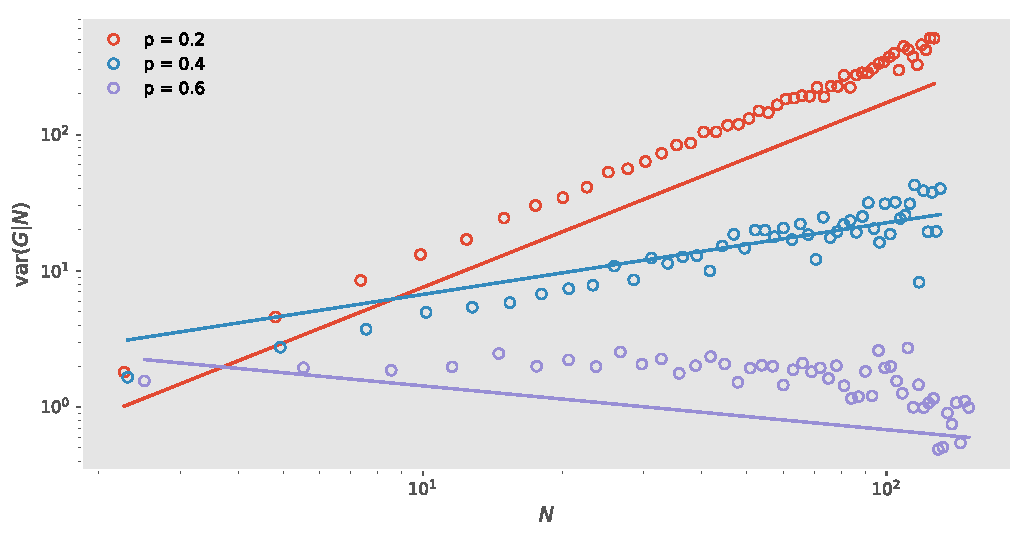
\includegraphics[scale=0.6]{figS1.pdf}
\caption{An illustration of the phase transition in Equation \ref{VGN}. }\label{fig:S1}
\end{figure}



\subsection{Broken state model}

Let the probability for a modified cell to break be $p$ and the probability for a broken cell to repair in a given generation be $q$. Letting $B_t$ and $G_t$ be the number of broken and green cells, we have
\begin{align}
M_t &= 2M_{t-1} -  \sum_{i}^{2M_{t-1}}\xi_{t,{\rm break},i}\\
B_t &= \sum_{i=1}^{B_{t-1}}(1-\xi_{t,{\rm repair},i}) + \sum_{i}^{2M_{t-1}}\xi_{t,{\rm break},i}\\
G_t &=2G_{t-1} + \sum_{i=1}^{B_{t-1}}\xi_{t,{\rm repair},i} 
\end{align}
where $\xi_{{\rm repair},i}$ and $\xi_{{\rm break},i}$ are $1$ if the $i$th cells in the sums are broken or repaired respectively, and zero otherwise. Making a Gaussian approximation, we have 
\begin{align}
\begin{split}\label{MBGt}
M_t &= 2M_{t-1}(1 - p)+ \sqrt{2p(1-p)M_{t-1}} \eta_{2,t}\\
B_t &= (1-q)B_{t-1} +2pM_{t-1} - \sqrt{q(1-q)B_{t-1}}\eta_{1,t} - \sqrt{2p(1-p)M_{t-1}} \eta_{2,t}\\
G_t &=2G_{t-1} + qB_{t-1}+\sqrt{q(1-q)B_{t-1}}\eta_{1,t}.
\end{split}
\end{align}
Here, $\eta_{i,t}$ are independent standard normal random variates, but note that we have been careful to flip the signs in-front of the noise terms above so that, e.g., a positive value of $\eta_{2,t}$ in the first equation corresponds to a negative value in the second. 

Conditioned on the previous generation, ${\bf z}_t = (M_t,B_t,G_t)^T$ has a multivariate Gaussian distribution: 
\begin{align}
f_t(\bz|\bz') = \frac{1}{\sqrt{2\pi } {\rm det}\Sigma_{t}(\bz')^{1/2}} e^{-\frac{1}{2}(\bz-\bmu_{t}(\bz'))^T\Sigma_{t}(\bz')^{-1}(\bz-\bmu_{t}(\bz'))}
\end{align}
The mean and covariance matrix can be determined from Equation \eqref{MBGt}. For the mean, we have
\begin{align}
\bmu_{t} &= \left[\begin{array}{c}
 \langle  M_t |\bz_{t-1}\rangle \\
 \langle  B_t |\bz_{t-1}\rangle \\
 \langle  G_t |\bz_{t-1}\rangle 
 \end{array}
\right]
%= \left[\begin{array}{c}
%2M_{t-1} -pM_{t-1}\\
%(1-q)B_{t-1} +pM_{t-1}\\
%2G_{t-1} + qB_{t-1}
%\end{array}
%\right]\\
%&
= A \bz_{t-1} 
\end{align}
where
\begin{equation}
A=\
\left[ \begin{array}{ccc}
2 -2p & 0 &0 \\
2p & 1-q & 0 \\
0 & q & 2
\end{array}\right].
\end{equation}
This leads to the recursive equation for the average:  
\begin{equation}
\langle \bz_t \rangle  = A \langle \bz_{t-1} \rangle 
\end{equation}
Taking the initial conditions to be $\bz_0 = (1,0,0)$ (that is, there is initially one modified cell), it is a straightforward exercise in linear algebra (or a few lines in Mathematica) to obtain 
\begin{equation}
\langle \bz_t \rangle  = \left[
\begin{array}{c}
 (2-2 p)^t \\
 \frac{2 p \left((1-q)^t-(2-2 p)^t\right)}{2 p-q-1} \\
 -\frac{q \left(2 p \left(2^t-(1-q)^t\right)+(q+1) 2^t \left((1-p)^t-1\right)\right)}{(q+1) (-2 p+q+1)} \\
\end{array}
\right].
\end{equation}
We find (as we could have deduced without this calculation) that the fraction of green cells approaches one as $t \to \infty$. 


Now we turn to the covariance matrix. The elements of $\Sigma_t$, are determined by variance and covariance of $B_t$ and $G_t$: 
\begin{align}
\begin{split}
\Sigma_{t,1,1} &= {\rm var}(M_t|\bz_{t-1}) =p(1-p)2M_{t-1}\\
\Sigma_{t,2,2} &= {\rm var}(B_t|\bz_{t-1}) = q(1-q)B_{t-1}+p(1-p)2M_{t-1}\\
\Sigma_{t,3,3} &= {\rm var}(G_t|\bz_{t-1}) = q(1-q)B_{t-1}
\end{split}
\end{align}
and 
\begin{align}
\begin{split}
\Sigma_{t,1,2} &={\rm cov}(M_t,B_t|\bz_{t-1}) = 2p(1-p)M_{t-1}\\
\Sigma_{t,2,3} &={\rm cov}(B_t,G_t|\bz_{t-1}) = q(1-q)B_{t-1}\\
\Sigma_{t,3,1} &={\rm cov}(M_t,G_t|\bz_{t-1}) = 0.
\end{split}
\end{align}
The covariance matrix is therefore, 
\begin{equation}
\Sigma_{t} =\left[ \begin{array}{ccc}
2p(1-p)M_{t-1}  & 2p(1-p)M_{t-1}  & 0\\
2p(1-p)M_{t-1}  & q(1-q)B_{t-1} + 2p(1-p)M_{t-1}  & q(1-q)B_{t-1} \\
0 &q(1-q)B_{t-1} & q(1-q)B_{t-1}
\end{array}\right].
\end{equation}

We are interested in the unconditional distribution $P_t(\bz)$, so we write the recursive equation
\begin{equation}
P_t(\bz) = \int f_t(\bz|\bz')P_{t-1}(\bz') d\bz'.
\end{equation}
We make ansatz that $P_t(\bz)$ is a Gaussian 
\begin{equation}
P_t(\bz) = \frac{1}{\sqrt{2\pi }\, \left[{\rm det}\Omega_{t}\right]^{1/2}} e^{-\frac{1}{2}(\bz-\bnu_{t})^T\Omega_{t}^{-1}(\bz-\bnu_{t})}.
\end{equation}
This is equivalent to assuming that $B_{t-1}$ and $G_{t-1}$ appearing in the elements of the covariance matrix can be replaced by their averages, thus making the joint distribution of $\bz$ and $\bz'$ also a multivariate Guassian. This allows us to write 
\begin{align}
\begin{split}
P_t(\bz,\bz') &= f_t(\bz|\bz')P_{t-1}(\bz') \propto e^{-\frac{1}{2}(\bz-\bmu_{t}(\bz'))^T\Sigma_{t}^{-1}(\bz-\bmu_{t}(\bz'))-\frac{1}{2}(\bz'-\bnu_{t-1})^T\Omega_{t-1}^{-1}(\bz'-\bnu_{t-1})}\\
&\propto e^{-\frac{1}{2}(\bz-\hat{\bmu}_t)^T\hat{\Sigma}_{t}^{-1}(\bz-\hat{\bmu}_{t})}
\end{split}
\end{align} 
where $\hat{\bmu}_t$ and $\hat{\Sigma}_{t}$ are the mean and covariance matrices of the joint distribution of the current and previous generations. 
%We match the matrix equations 
%\begin{equation}
%((\bz,\bz')-\hat{\bmu}_t)^T\hat{\Sigma}_{t}^{-1}((\bz,\bz')-\hat{\bmu}_{t}) = (\bz-\bmu_{t}(\bz'))^T\Sigma_{t}^{-1}(\bz-\bmu_{t}(\bz'))+(\bz'-\bnu_t)^T\Omega_t^{-1}(\bz'-\bnu_t) 
%\end{equation}
Since $\bz$ and $\bz'$ have marginal distributions given by  $P_{t}(\bz)$ and $P_{t-1}(\bz)$ respectively, $\hat{\Sigma}_{t}$ has the block form:
\begin{equation}
\hat{\Sigma}_{t} = \left[ \begin{array}{cc}
\Omega_t  & U_t\\
U_t^T  &\Omega_{t-1} 
\end{array}\right].
\end{equation}
where 
\begin{equation}
U_t =\left[ \begin{array}{ccc}
{\rm cov}(M_t,M_{t-1})  &{\rm cov}(M_t,B_{t-1})  &{\rm cov}(M_t,G_{t-1}) \\
{\rm cov}(B_t,M_{t-1})  &{\rm cov}(B_t,B_{t-1})  &{\rm cov}(B_t,G_{t-1}) \\
{\rm cov}(G_t,M_{t-1})  &{\rm cov}(G_t,B_{t-1})  &{\rm cov}(G_t,G_{t-1}) 
\end{array}\right].
\end{equation}
%Let's work out the elements of this covariance matrix. Starting with the diagonal entries:
%\begin{align}
%\begin{split}
%{\rm cov}(M_t,M_{t-1})  &= 2 {\rm var}(M_{t-1})\\
%{\rm cov}(B_t,B_{t-1}) &= (1-q){\rm var}(B_{t-1}) + 2p {\rm cov}(B_{t-1},M_{t-1})\\
%{\rm cov}(G_t,G_{t-1}) &=  2{\rm var}(G_{t-1}) + q {\rm cov}(G_{t-1},B_{t-1})\\
%{\rm cov}(M_t,B_{t-1}) &= 2 {\rm cov}(M_{t-1},B_{t-1})\\
%{\rm cov}(M_t,G_{t-1}) &= 2 {\rm cov}(M_{t-1},G_{t-1})\\
%{\rm cov}(B_t,G_{t-1}) &=(1-q){\rm cov}(B_{t-1},G_{t-1}) + 2p {\rm cov}(M_{t-1},G_{t-1})\\
%{\rm cov}(B_t,M_{t-1}) &= 2(1-q){\rm cov}(B_{t-1},M_{t-1}) + 2 p {\rm var}(M_{t-1})\\
%{\rm cov}(G_t,M_{t-1}) &= 2 {\rm cov}(G_{t-1},M_{t-1}) + q {\rm cov}(B_{t-1},M_{t-1})\\
%{\rm cov}(G_t,B_{t-1}) &= 2 {\rm cov}(G_{t-1},B_{t-1}) + q{\rm var}(B_{t-1})
%\end{split}
%\end{align}
After some algebra, we find that we can write the matrices $U_t$ in terms of the entries of $\Omega_{t-1}$ (dropping the time subscript for clarity): 
\begin{align}
U_t &=\left[ \begin{array}{ccc}
2(1-p)\Omega_{1,1}  & 2(1-p) \Omega_{1,2}  & 2(1-p) \Omega_{t-1,1,3} \\
(1-q) \Omega_{2,1} + 2 p \Omega_{1,1}&(1-q)\Omega_{2,2} + 2p \Omega_{1,2}  &(1-q) \Omega_{2,3} + 2p \Omega_{1,3}\\
2\Omega_{3,1} + q \Omega_{2,1} &2 \Omega_{3,2} + q \Omega_{2,2}  &2\Omega_{3,3} + q \Omega_{3,2}
\end{array}\right]\\
&= D\Omega_{t-1}
\end{align}
where
\begin{equation}
D = \left[ \begin{array}{ccc}
2(1-p)  &0  &0 \\
2p  & (1-q)  & 0 \\
0 & q  &2
\end{array}\right].
\end{equation}
In order to derive an equation for $\Omega_t$, we notice that standard properties of multivariate normal distributions allow us to write $\Sigma_t$ (which is known) as a Shur complement of the blocks in $\hat{\Sigma}$:
 \begin{equation}
 \Sigma_t = \Omega_{t} - U_t \Omega_{t-1}^{-1}U_t^T\
 \end{equation}
 which gives us a recursive relation for $\Omega_t$: 
 \begin{equation}
 \Omega_{t} =  \Sigma_t + D(D\Omega_{t-1})^T =  \Sigma_t + D\Omega_{t-1}D^T
 \end{equation}
 Taking $\Omega_{0}$ to be a matrix of all zeros, 
 \begin{equation}
  \Omega_{t} = \sum_{j\le t}D^{t-j}\Sigma_j \left(D^T\right)^{t-j}
 \end{equation}
 
 
\begin{figure}[h!]
\centering
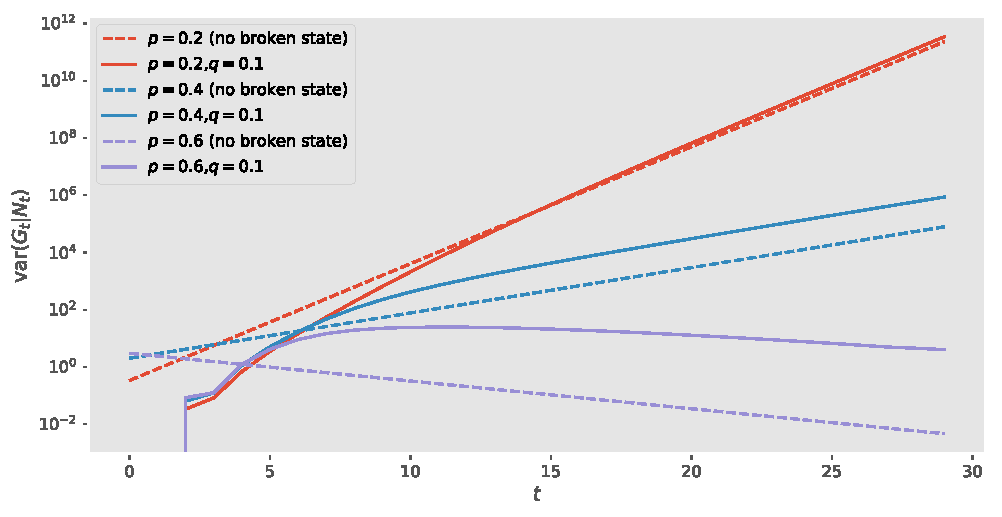
\includegraphics[scale=0.6]{figS2.pdf}
\caption{ Theoretical predictions for the growth of ${\rm var}(G|N)$ for the model with a broken state using Equation \ref{VGN_broken} compared to the predictions for a model with no broken state (Equation \ref{VGN}).  }\label{fig:S2}
\end{figure}

 We are actually interested in the variation in green cells conditioned on the total number of cells, thus, we introduce the transformation 
 \begin{equation}
 L = \left[ \begin{array}{ccc}
1  & 1 &1 \\
0  & 0& 1 \\
\end{array}\right].
 \end{equation} 
 This gives us the covariance matrix for $(N_t,G_t)$:
 \begin{equation}
  \bar{\Omega}_{t} =L\Omega_t L^T =  \sum_{j\le t}LD^{t-j}\Sigma_j \left(D^T\right)^{t-j}L^T
 \end{equation}
 In terms of the entries of $ \tilde{\Omega}_{t}$, 
 \begin{equation}\label{VGN_broken}
 {\rm var}(G_t|N_t) = \bar{\Omega}_{t,2,2} - \frac{\bar{\Omega}_{t,1,2}^2}{ \bar{\Omega}_{t,1,1} }. 
 \end{equation}
Although we don't have a closed form for ${\rm var}(G_t|N_t)$, it can easily be computed numerically. We find that the broken state seems to have no effect on the long term growth of  ${\rm var}(G_t|N_t)$; see Figure \ref{fig:S2}. 






\bibliographystyle{plain}
\bibliography{/Users/E/Dropbox/bib/main.bib}


\end{document}  